\begin{table}[H]
\centering
\definecolor{tabglobaljointnorm0}{rgb}{1.0,1.0,0.8}
\definecolor{tabglobaljointnorm1}{rgb}{0.9961,0.797,0.4046}
\definecolor{tabglobaljointnorm2}{rgb}{0.993,0.5825,0.2481}
\definecolor{tabglobaljointnorm3}{rgb}{0.9961,0.7778,0.3839}
\definecolor{tabglobaljointnorm4}{rgb}{0.9921,0.5491,0.2342}
\definecolor{tabglobaljointnorm5}{rgb}{0.9961,0.7346,0.3374}
\definecolor{tabglobaljointnorm6}{rgb}{0.991,0.4793,0.2143}
\definecolor{tabglobaljointnorm7}{rgb}{0.9944,0.6372,0.2717}
\definecolor{tabglobaljointnorm8}{rgb}{0.9832,0.2955,0.1619}
\definecolor{tabglobaljointnorm9}{rgb}{0.9928,0.578,0.2461}
\definecolor{tabglobaljointnorm10}{rgb}{0.8072,0.0452,0.1316}
\definecolor{tabglobaljointnorm11}{rgb}{0.9925,0.5643,0.2402}
\definecolor{tabglobaljointnorm12}{rgb}{0.502,0.0,0.149}
\definecolor{tabglobaljointnorm13}{rgb}{0.9906,0.4561,0.2076}
\definecolor{tabglobaljointnorm14}{rgb}{1.0,0.9801,0.7513}
\definecolor{tabglobaljointnorm15}{rgb}{1.0,0.9402,0.6538}
\definecolor{tabglobaljointnorm16}{rgb}{0.9984,0.8971,0.5596}
\definecolor{tabglobaljointnorm17}{rgb}{0.9961,0.8498,0.4615}
\definecolor{tabglobaljointnorm18}{rgb}{0.9961,0.7634,0.3684}
\definecolor{tabglobaljointnorm19}{rgb}{0.9955,0.6781,0.2894}
\definecolor{tabglobaljointnorm20}{rgb}{0.9933,0.5962,0.254}
\definecolor{tabglobaljointnorm21}{rgb}{0.9888,0.3398,0.1744}
\definecolor{tabglobaljointnorm22}{rgb}{0.9463,0.2187,0.1412}
\definecolor{tabglobaljointnorm23}{rgb}{0.8867,0.0996,0.1107}
\definecolor{tabglobaljointnorm24}{rgb}{0.8025,0.042,0.1329}
\definecolor{tabglobaljointnorm25}{rgb}{0.7046,0.0,0.149}
\definecolor{tabglobaljointnorm26}{rgb}{0.5695,0.0,0.149}
\begin{minipage}{0.78\textwidth}
\centering
\renewcommand{\arraystretch}{1.2}
\begin{tabular}{lccc}
\toprule
Checkpoint & First & Middle & Last \\
\midrule
0 & \cellcolor{tabglobaljointnorm0}\textcolor{black}{$0.000 \pm 0.000$} & \cellcolor{tabglobaljointnorm1}\textcolor{black}{$0.124 \pm 0.098$} & \cellcolor{tabglobaljointnorm2}\textcolor{black}{$0.201 \pm 0.078$} \\
1 & \cellcolor{tabglobaljointnorm0}\textcolor{black}{$0.000 \pm 0.000$} & \cellcolor{tabglobaljointnorm3}\textcolor{black}{$0.130 \pm 0.097$} & \cellcolor{tabglobaljointnorm4}\textcolor{black}{$0.211 \pm 0.077$} \\
5 & \cellcolor{tabglobaljointnorm0}\textcolor{black}{$0.000 \pm 0.000$} & \cellcolor{tabglobaljointnorm5}\textcolor{black}{$0.146 \pm 0.094$} & \cellcolor{tabglobaljointnorm6}\textcolor{black}{$0.226 \pm 0.075$} \\
15 & \cellcolor{tabglobaljointnorm0}\textcolor{black}{$0.000 \pm 0.000$} & \cellcolor{tabglobaljointnorm7}\textcolor{black}{$0.181 \pm 0.090$} & \cellcolor{tabglobaljointnorm8}\textcolor{white}{$0.267 \pm 0.068$} \\
50 & \cellcolor{tabglobaljointnorm0}\textcolor{black}{$0.000 \pm 0.000$} & \cellcolor{tabglobaljointnorm9}\textcolor{black}{$0.203 \pm 0.084$} & \cellcolor{tabglobaljointnorm10}\textcolor{white}{$0.346 \pm 0.052$} \\
200 & \cellcolor{tabglobaljointnorm0}\textcolor{black}{$0.000 \pm 0.000$} & \cellcolor{tabglobaljointnorm11}\textcolor{black}{$0.207 \pm 0.076$} & \cellcolor{tabglobaljointnorm12}\textcolor{white}{$0.421 \pm 0.039$} \\
last & \cellcolor{tabglobaljointnorm0}\textcolor{black}{$0.000 \pm 0.000$} & \cellcolor{tabglobaljointnorm13}\textcolor{black}{$0.232 \pm 0.076$} & \cellcolor{tabglobaljointnorm12}\textcolor{white}{$0.422 \pm 0.033$} \\
\bottomrule
\end{tabular}
\end{minipage}%
\hfill
\begin{minipage}{0.15\textwidth}
\centering
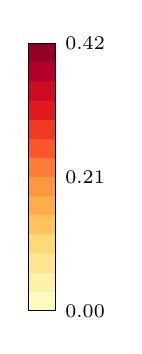
\begin{tikzpicture}
\fill[tabglobaljointnorm14] (0,0.0000) rectangle (0.35,0.2429);
\fill[tabglobaljointnorm15] (0,0.2429) rectangle (0.35,0.4857);
\fill[tabglobaljointnorm16] (0,0.4857) rectangle (0.35,0.7286);
\fill[tabglobaljointnorm17] (0,0.7286) rectangle (0.35,0.9714);
\fill[tabglobaljointnorm18] (0,0.9714) rectangle (0.35,1.2143);
\fill[tabglobaljointnorm19] (0,1.2143) rectangle (0.35,1.4571);
\fill[tabglobaljointnorm20] (0,1.4571) rectangle (0.35,1.7000);
\fill[tabglobaljointnorm6] (0,1.7000) rectangle (0.35,1.9429);
\fill[tabglobaljointnorm21] (0,1.9429) rectangle (0.35,2.1857);
\fill[tabglobaljointnorm22] (0,2.1857) rectangle (0.35,2.4286);
\fill[tabglobaljointnorm23] (0,2.4286) rectangle (0.35,2.6714);
\fill[tabglobaljointnorm24] (0,2.6714) rectangle (0.35,2.9143);
\fill[tabglobaljointnorm25] (0,2.9143) rectangle (0.35,3.1571);
\fill[tabglobaljointnorm26] (0,3.1571) rectangle (0.35,3.4000);
\draw[black,line width=0.3pt] (0,0) rectangle (0.35,3.4000);
\node[right,font=\scriptsize,anchor=west] at (0.35,3.4000) {0.42};
\node[right,font=\scriptsize,anchor=west] at (0.35,1.7000) {0.21};
\node[right,font=\scriptsize,anchor=west] at (0.35,0) {0.00};
\end{tikzpicture}
\end{minipage}
\caption{Global Wasserstein alignment, JointSheafParams (identity init), normalised. Mean $\pm$ SE across 9 datasets (First/Last), 7 for Middle (datasets with $L=2$ contribute no middle layer). Tolokers is excluded: training was unstable for this configuration (JointSheafParams, normalised=True) and no reference profile was saved. (Pooled fold/layer SE averages 0.017 across cells; not shown per cell, see text.) Cell shading: white = 0, dark red = 0.42 (max value in this table), YlOrRd colormap, same scale as Fig.~\ref{fig: RM_Norm} etc.}
\label{tab:global_joint_norm}
\end{table}
